\section{Energetic Results}
\label{sec:energetic}

In order to analyse the energetic costs of the \ac{BLE} system implementation a series of tests were planned and executed. The tests were divided into three categories, system off, system on and system working, presented in sections \ref{subsec:syson}, \ref{subsec:sysoff} and \ref{subsec:syswork}, respectfully. With this analysis one intends to understand the energetic cost of a smartphone on standby, in order to comprehend the baseline consumption and compare it with the energetic costs of the application, in multiple tests with varying elements. 

The utilised smartphone was a Sony Xperia E5, whose battery is rated at 2300 mAh. The battery values data collection was made through the android api which allows one to know the battery percentage of the smartphone. As such all the collected values have a constant error margin of 1 percent of the total battery, i.e. 23 mAh.

The tests were all conducted under the same base conditions, the battery was completely charged, without a SIM card and with the screen at maximum brightness. They were also conducted over the period of an hour.

\subsection{System Off}
\label{subsec:syson}

This category includes one single text case, case number 1, and its intention was to analyse the smartphone's energy consumption on standby with its system turned off. This case's test conditions were having Wi-Fi and Bluetooth turned off and leaving the screen active on the main screen.

The test results can be seen on figure \ref{fig:sysoff} and show the battery capacity's progress over the test duration. From this we can assume that the standby energetic cost of the used smartphone is [138 +/- 23] and use it as a baseline for the remaining cost comparisons.

\begin{figure}
	\centering
		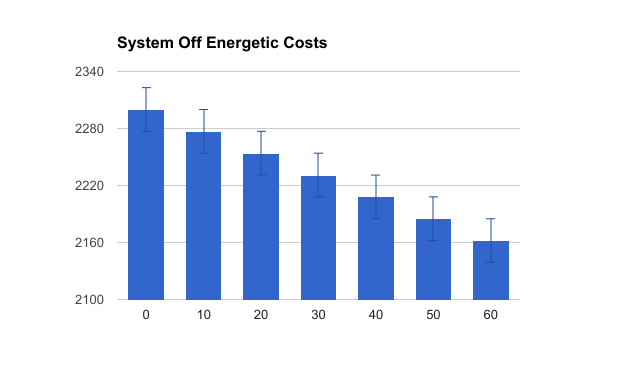
\includegraphics[width=0.5\linewidth]{5.Chapter/system-off.png}
	\caption[Test case #1: System Off - energetic costs]{Test case #1: System Off - energetic costs}
	\label{fig:sysoff}
\end{figure}


\subsection{System On}
\label{subsec:sysoff}

In this category one will study the energetic impact of Wi-Fi and Bluetooth on the smartphone device. In order to do so, three tests were conducted: The first one (test case #2), activates the Wi-Fi without having available service; The second one (test case #3), activetes the Wi-Fi while providing service; And the last one (test case #4), allows the same Wi-Fi conditions from the previous test (test case #3) while activating bluetooth and using the implemented application with a five second discovery cycle without any nearby compatible \ac{BLE} devices.

The energetic cost's comparison of these three test cases and the one presented in section \ref{subsec:syson}, which is used for a standby comparison, can be seen on figure \ref{fig:syson}. The presented figure allows one to visualize the overall energetic impact of the smartphone's sensors, which would be around [23 +/- 11.5] mAh, equivalent to one percent of the smartphone's battery.

\begin{figure}
	\centering
		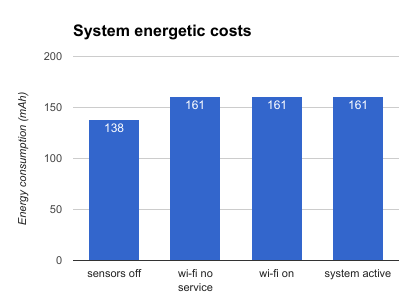
\includegraphics[width=0.5\linewidth]{5.Chapter/system-on.png}
	\caption[Test case #2,3,4: System On - energetic costs]{Test case #2,3,4: System On - energetic costs}
	\label{fig:syson}
\end{figure}

\subsection{System Working}
\label{subsec:syswork}

In this category one will study the energetic impact of the indoor location application on the smartphone. In order to do so, tests were conducted where two parameters were tuned, the number of nearby beacons and the discovery proccedure frequency. The discovery period was tuned using four different values, five, fifteen, thirty and sixty seconds, while the number of nearby beacons was either one or two. Using all the possible parameters combinations, eight test cases were conducted, which can be visualised on figure \ref{fig:syswork}.

\begin{figure}
	\centering
		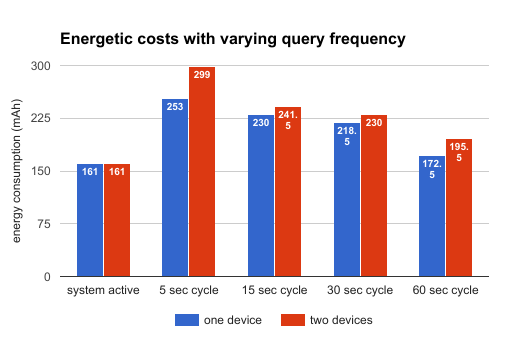
\includegraphics[width=0.5\linewidth]{5.Chapter/system-working.png}
	\caption[Test case #5-12: System Working - energetic costs]{Test case #5-12: System Working - energetic costs}
	\label{fig:syswork}
\end{figure}

Tests cases #4 is shown in order to establish as a reference the minimum energetic cost of the application. The remaining data is grouped into pairs, with each pair having in common the used discovery proccedure period. Test case #5 and #6 use 5 seconds cycles, cases #7 and #8 use 15 seconds, cases #9 and #10 use 30 seconds and cases #11 and #12 use 60 seconds.

From the displayed graphic we can the energetic impact that occurs when adding an extra \ac{BLE} device for the application to interact with. The existance of more than one device leads to an energetic increase in two areas of the application. The first happens in the \ac{BLE} communication, where the mobile application has to communicate with each nearby \ac{BLE} devices and as such the cost of this operation is proportionate to the number of existant nearby tags. The second occurs on the part where the smartphone application communicates with the maps server. In the implemented system, the maps are provided through google maps, and as such in the scenario where there is only one beacon, i.e. the location obtained remains the same for the whole duration of the test, the cost are reduced since the maps isn't required to be updated. In the presence of two or more nearby beacons, if one considers the case where the location is constantly changing, each cycle implies that other than the constant communication cost with google maps, there is also need to update the map. The test cases using two beacons were made such that both were in the same place, one over the other, and the \ac{RSSI} variation characteristic was used to make sure the resulting location wouldn't be constant over the course of the hour. Since the read values would vary in such a big manner, the cell with the strongest signal would change frequently, explaining the cost difference between the test cases with one and two devices.